\documentclass[superscriptaddress, twocolumn, prl]{revtex4}

\usepackage{amsmath}    % need for subequations
\usepackage[pdftex]{graphicx}   % need for figures
\usepackage{verbatim}   % useful for program listings
\usepackage{color}      % use if color is used in text
\usepackage{subfigure}  % use for side-by-side figures
\usepackage{hyperref}   % use for hypertext links, including those to external documents and URLs
\allowdisplaybreaks

\begin{document}
\appendix
\section{\label{App:add_data}Appendix: Cost Function and Additional Data}
\begin{align*}
\label{eq:cost}
\Delta x_{i_{c}} &= \left\vert f_{1,i_{c}}-\frac{f_{1,i_{c}}+m\left(c,\gamma\right)f_{2,i_{c}}}{m\left(c,\gamma\right)^{2}+1}\right\vert
\\ \Delta y_{i_c} &= \left\vert f_{2,i_{c}}-\frac{m\left(c,\gamma\right)\left(f_{1,i_{c}}+m\left(c,\gamma\right)f_{2,i_{c}}\right)}{m\left(c,\gamma\right)^{2}+1}  \right\vert
\\ C\left(\gamma\right) &= \sum_{c}\frac{1}{N_{c}}\sum_{i_c=1}^{N_{c}}\left(\Delta x_{i_c}\right)^{2}+\left(\Delta y_{i_c}\right)^{2}
\end{align*}

$\Delta x_{i_c}$ and $\Delta y_{i_c}$ are the respective horizontal and vertical distances of the $i^{th}$ point in cluster $c$ to its assigned line, and $N_{c}$ is the number of points in cluster $c$. Each cluster $c$ corresponds to one type of mode transition $n \rightarrow n\pm1$.

\begin{figure*}[ht]
\centering
\subfigure{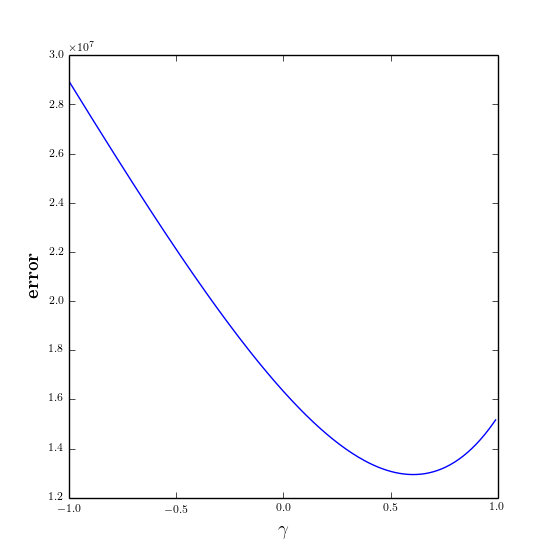
\includegraphics[width=\columnwidth]{error_V1.png}}
\subfigure{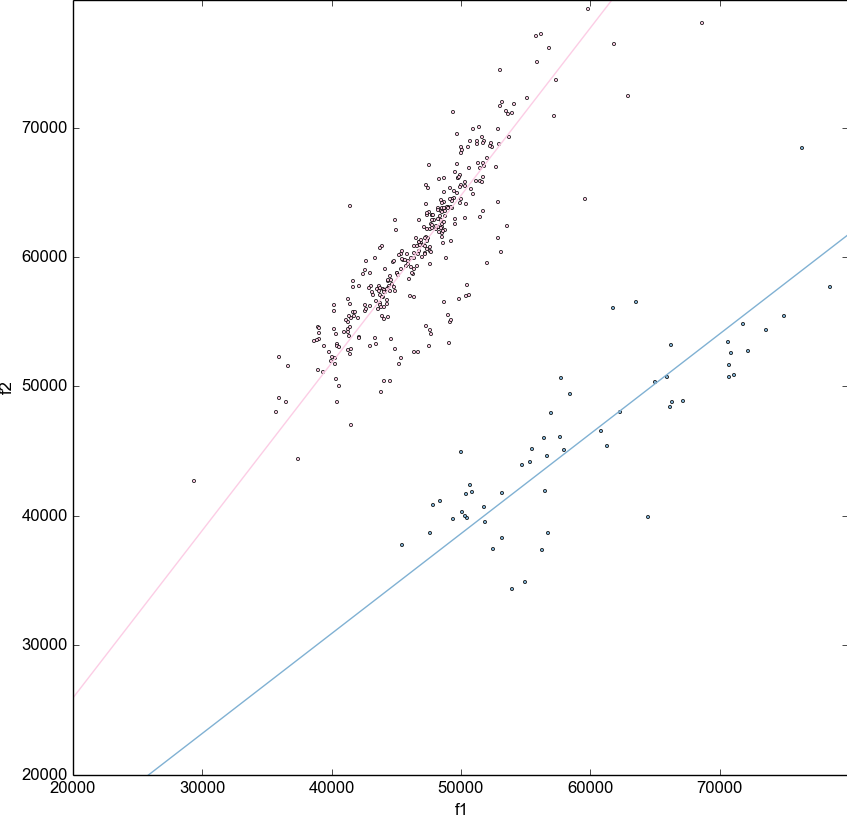
\includegraphics[width=\columnwidth]{V1.png}}
\caption{For rat V1, left shows plot of $C\left(\gamma \right)$ as a function of $\gamma$. Right shows output of clustering algorithm with $\gamma$ equal to the value shown in Fig. \ref{fig:gamma_error}.}
\end{figure*}

\begin{figure*}[h]
\centering
\subfigure{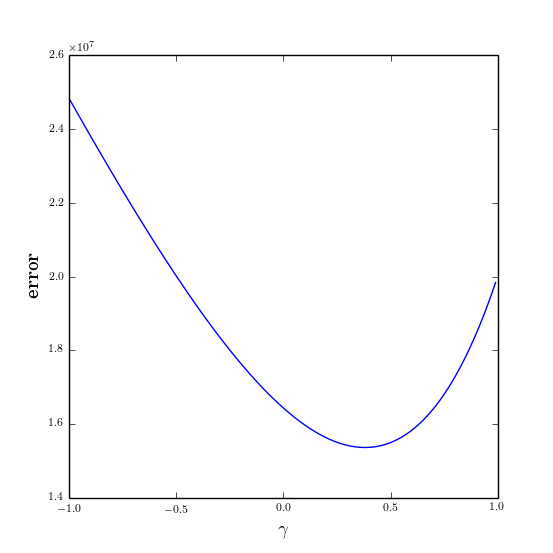
\includegraphics[width=\columnwidth]{error_V2.png}}
\subfigure{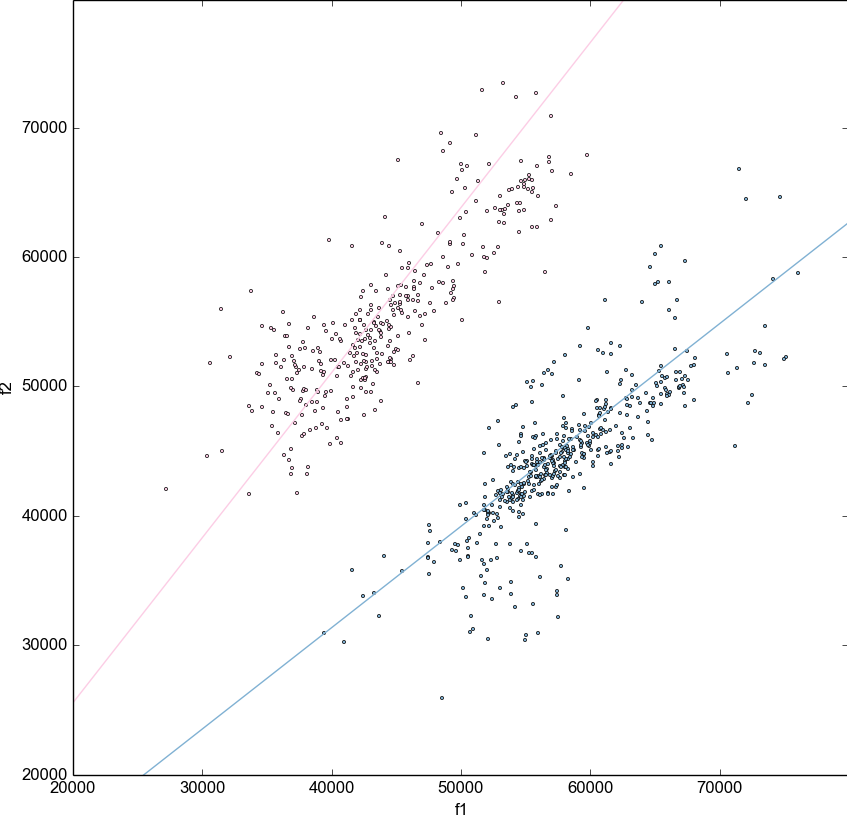
\includegraphics[width=\columnwidth]{V2.png}}
\caption{For rat V2, left shows plot of $C\left(\gamma \right)$ as a function of $\gamma$. Right shows output of clustering algorithm with $\gamma$ equal to the value shown in Fig. \ref{fig:gamma_error}.}
\end{figure*}

\begin{figure*}
\centering
\subfigure{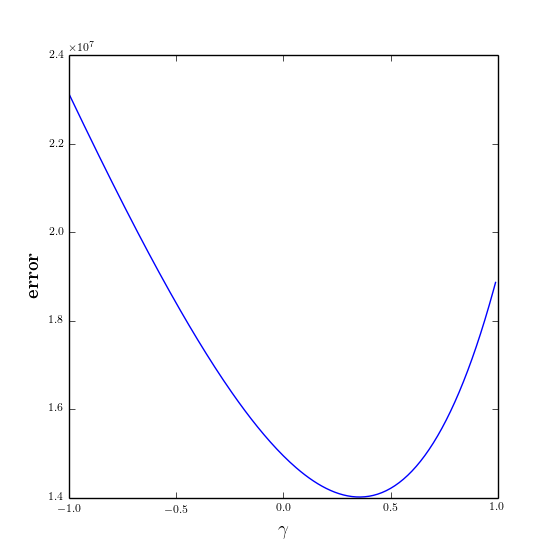
\includegraphics[width=\columnwidth]{error_V3.png}}
\subfigure{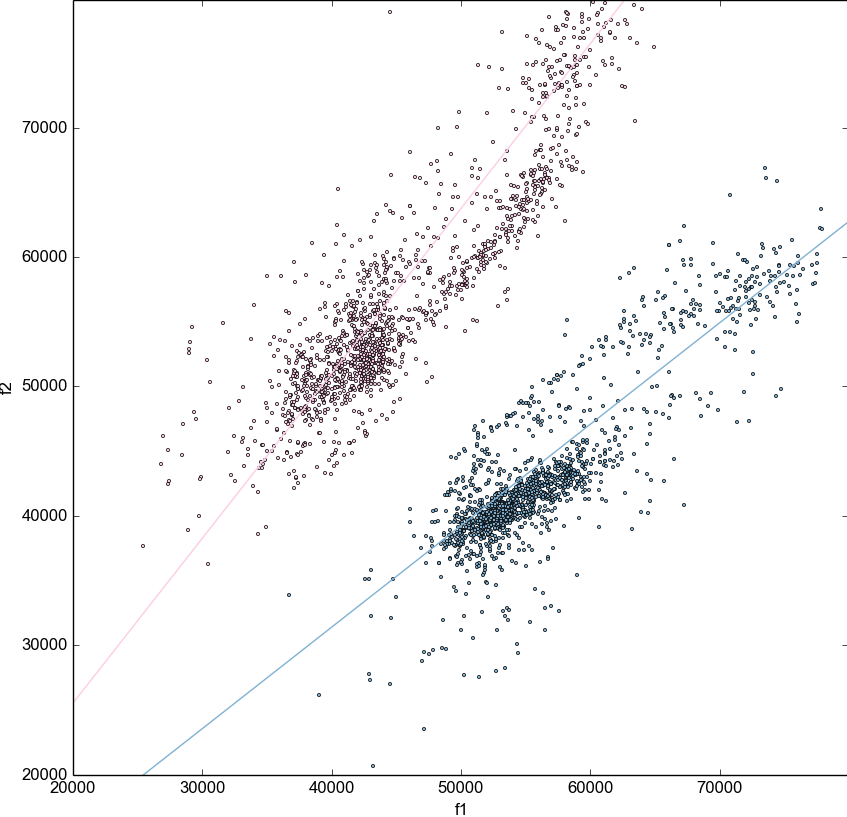
\includegraphics[width=\columnwidth]{V3.png}}
\caption{For rat V3, left shows plot of $C\left(\gamma \right)$ as a function of $\gamma$. Right shows output of clustering algorithm with $\gamma$ equal to the value shown in Fig. \ref{fig:gamma_error}.}
\end{figure*}

\begin{figure*}
\centering
\subfigure{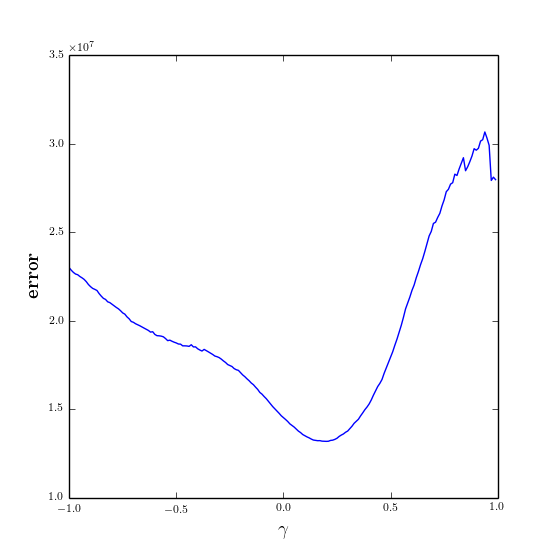
\includegraphics[width=\columnwidth]{error_V4.png}}
\subfigure{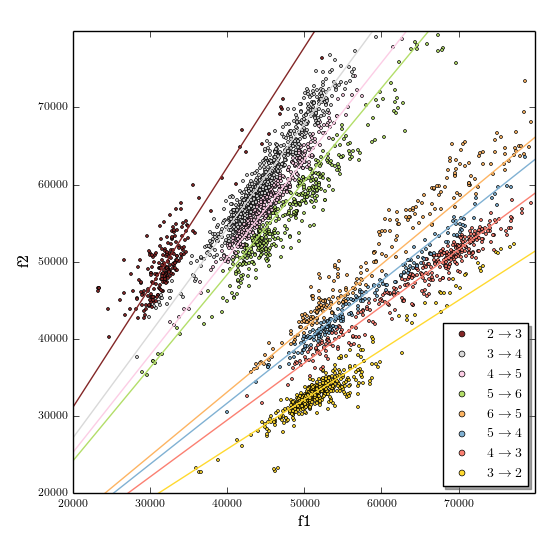
\includegraphics[width=\columnwidth]{V4.png}}
\caption{For rat V4, left shows plot of $C\left(\gamma \right)$ as a function of $\gamma$. Right shows output of clustering algorithm with $\gamma$ equal to the value shown in Fig. \ref{fig:gamma_error}.}
\end{figure*}

\begin{figure*}
\centering
\subfigure{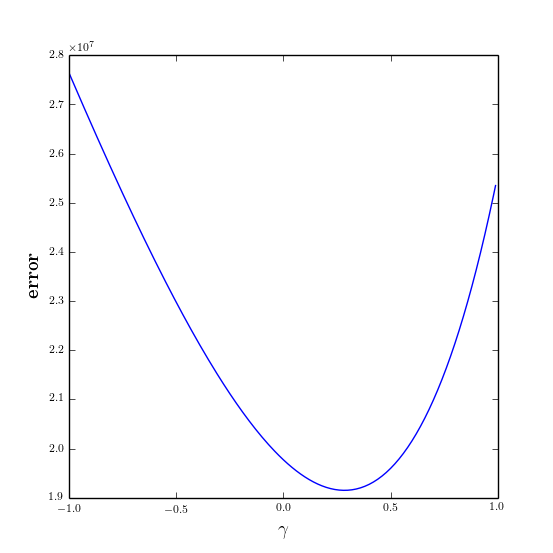
\includegraphics[width=\columnwidth]{error_V5.png}}
\subfigure{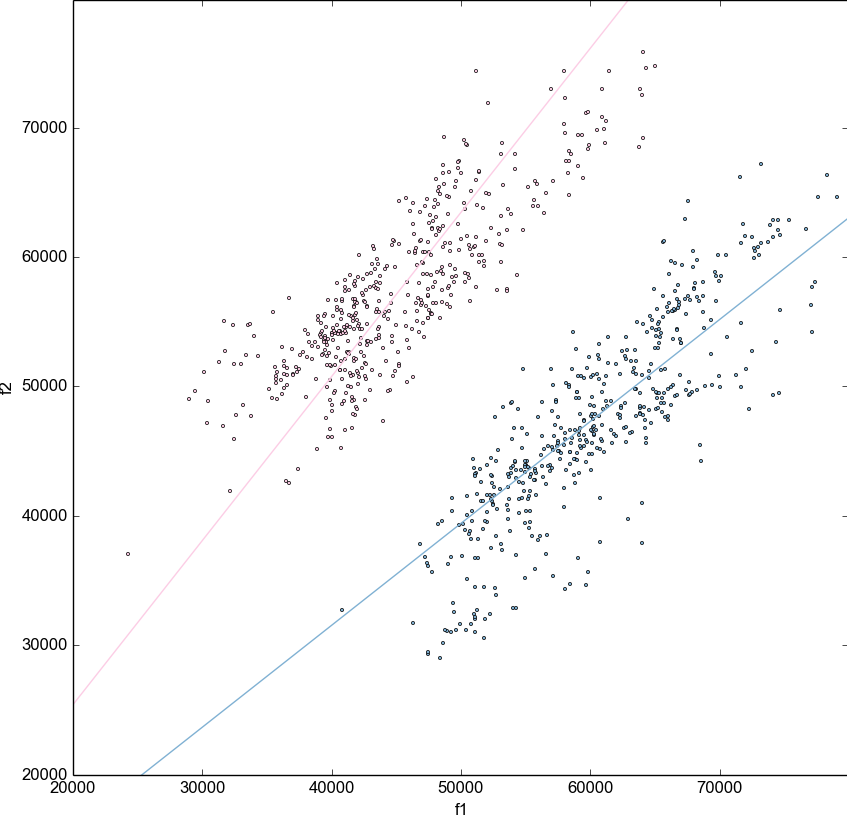
\includegraphics[width=\columnwidth]{V5.png}}
\caption{For rat V5, left shows plot of $C\left(\gamma \right)$ as a function of $\gamma$. Right shows output of clustering algorithm with $\gamma$ equal to the value shown in Fig. \ref{fig:gamma_error}.}
\end{figure*}

\begin{figure*}
\centering
\subfigure{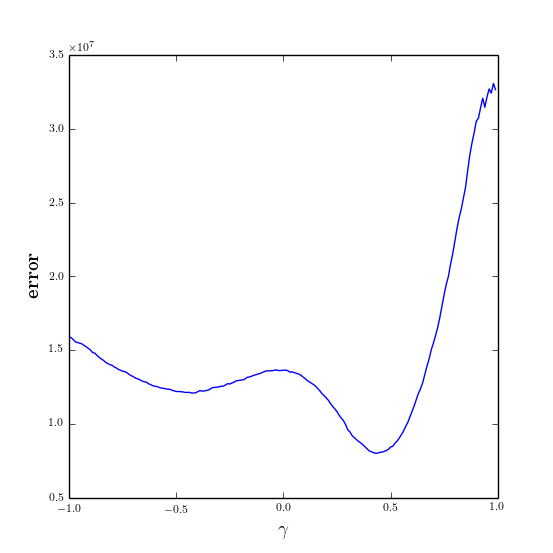
\includegraphics[width=\columnwidth]{error_V6.png}}
\subfigure{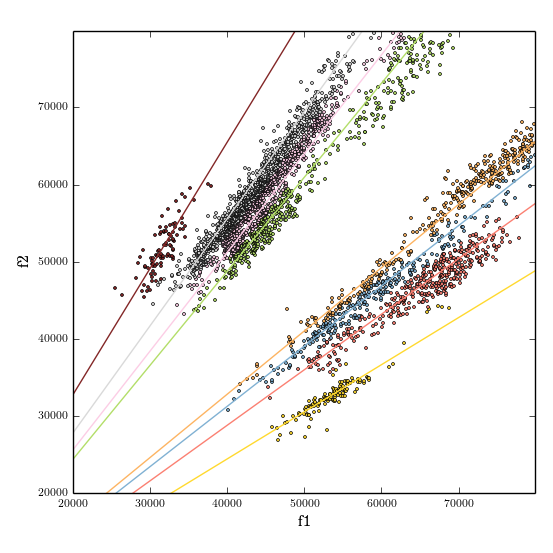
\includegraphics[width=\columnwidth]{V6.png}}
\caption{For rat V6, left shows plot of $C\left(\gamma \right)$ as a function of $\gamma$. Right shows output of clustering algorithm with $\gamma$ equal to the value shown in Fig. \ref{fig:gamma_error}.}
\end{figure*}

\begin{figure*}
\centering
\subfigure{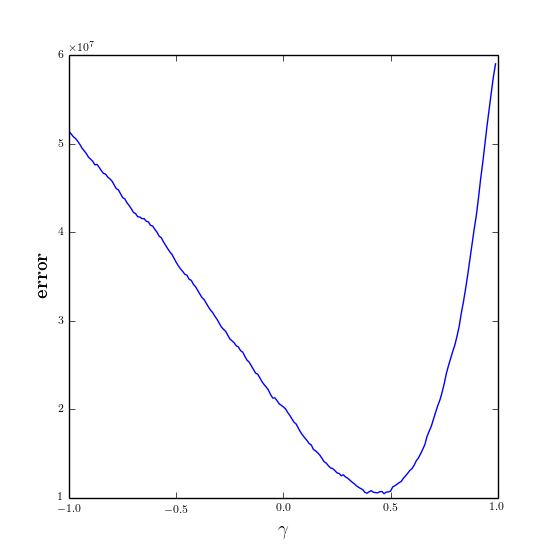
\includegraphics[width=\columnwidth]{error_V15.png}}
\subfigure{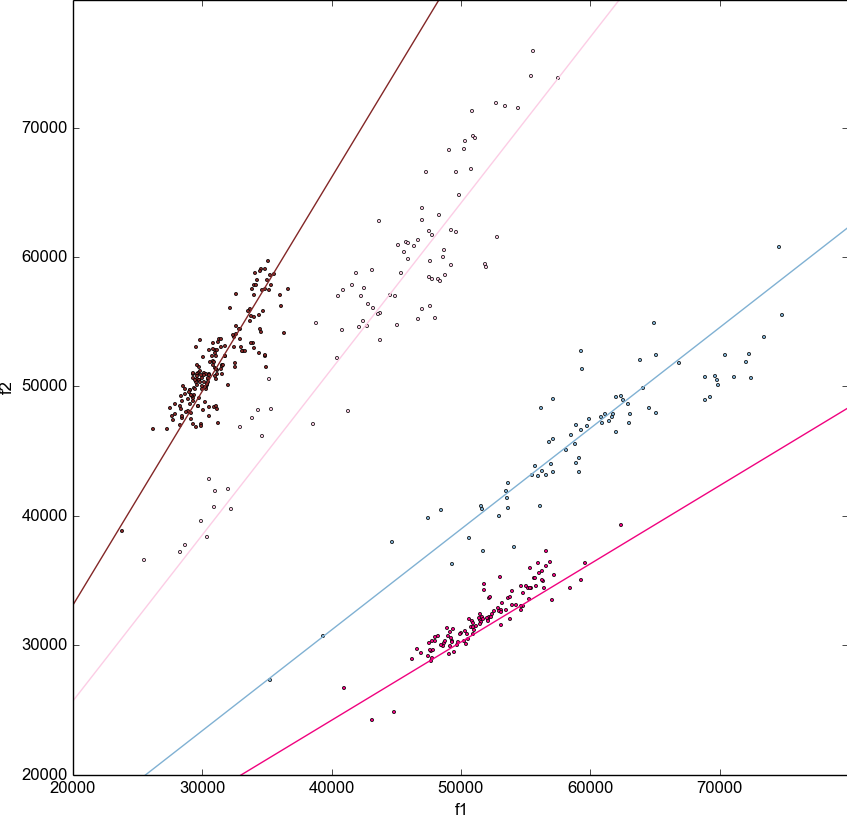
\includegraphics[width=\columnwidth]{V15.png}}
\caption{For rat V15, left shows plot of $C\left(\gamma \right)$ as a function of $\gamma$. Right shows output of clustering algorithm with $\gamma$ equal to the value shown in Fig. \ref{fig:gamma_error}.}
\end{figure*}

\begin{figure*}
\centering
\subfigure{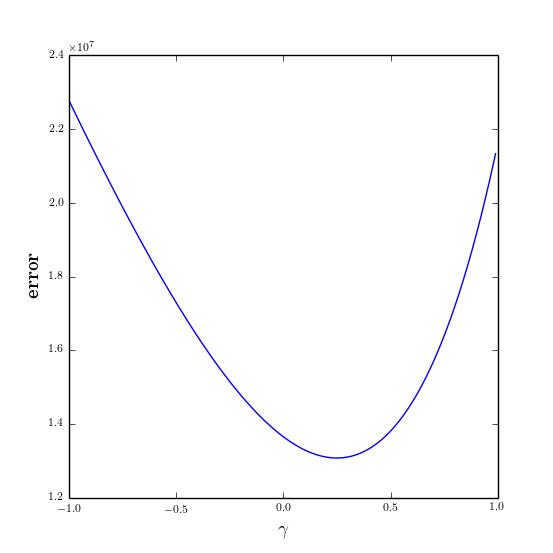
\includegraphics[width=\columnwidth]{error_V17.png}}
\subfigure{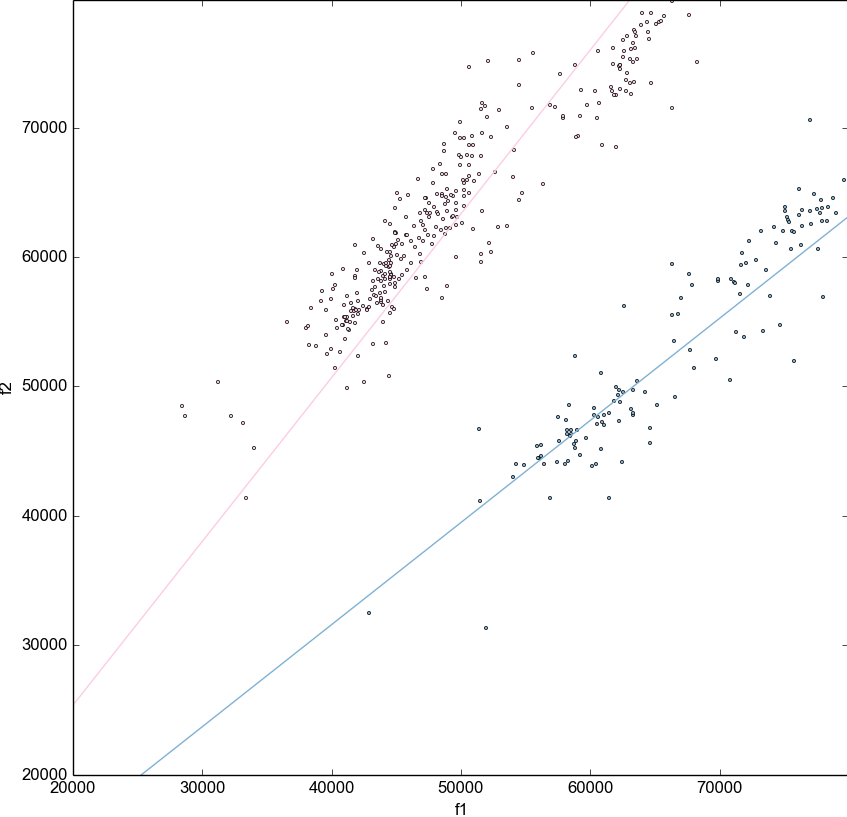
\includegraphics[width=\columnwidth]{V17.png}}
\caption{For rat V17, left shows plot of $C\left(\gamma \right)$ as a function of $\gamma$. Right shows output of clustering algorithm with $\gamma$ equal to the value shown in Fig. \ref{fig:gamma_error}.}
\end{figure*}

\begin{figure*}
\centering
\subfigure{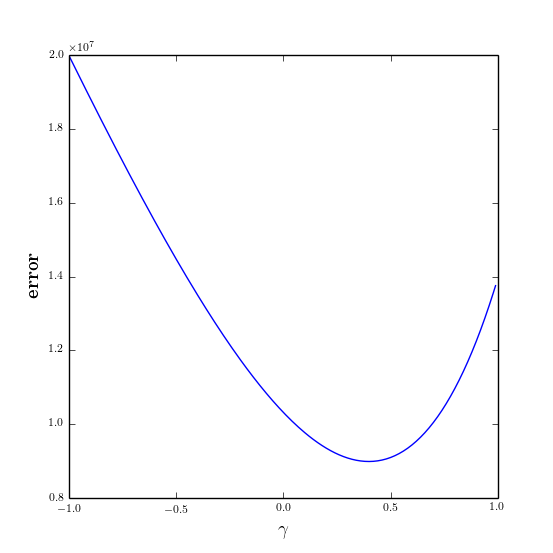
\includegraphics[width=\columnwidth]{error_V18.png}}
\subfigure{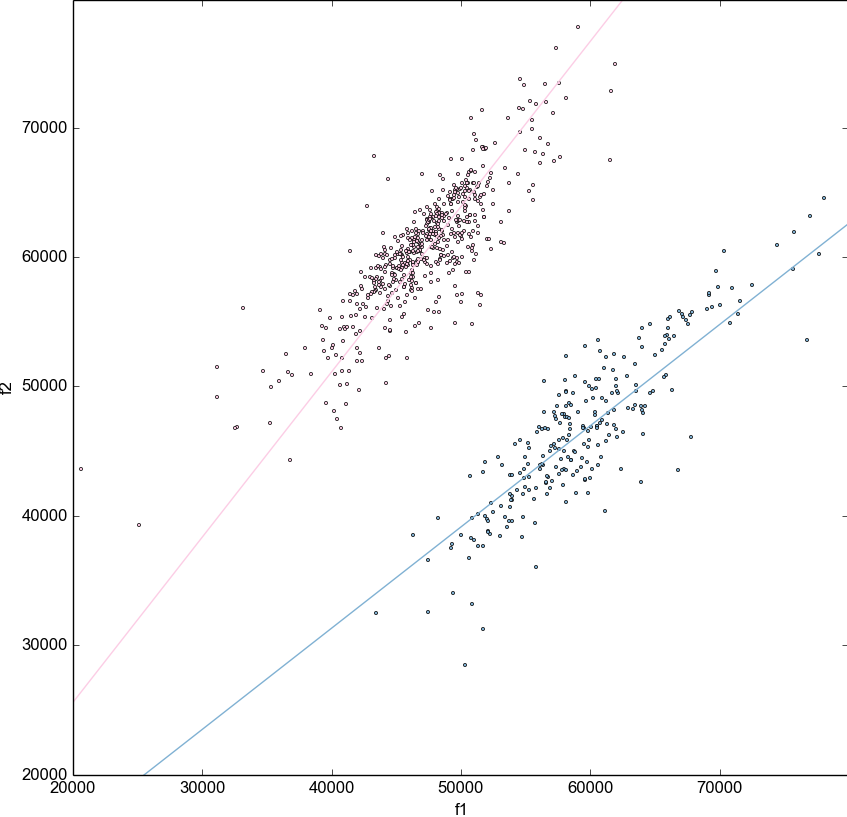
\includegraphics[width=\columnwidth]{V18.png}}
\caption{For rat V18, left shows plot of $C\left(\gamma \right)$ as a function of $\gamma$. Right shows output of clustering algorithm with $\gamma$ equal to the value shown in Fig. \ref{fig:gamma_error}.}
\end{figure*}

\begin{figure*}
\centering
\subfigure{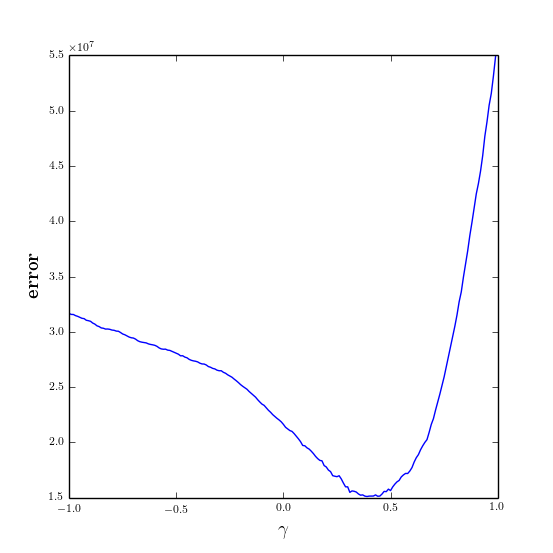
\includegraphics[width=\columnwidth]{error_V31.png}}
\subfigure{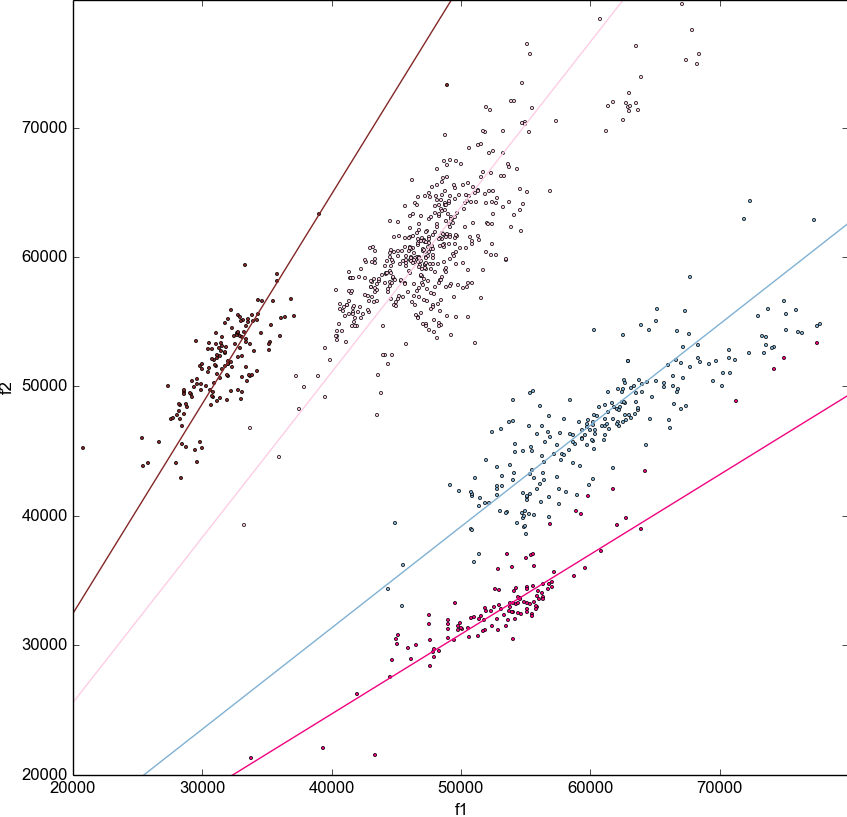
\includegraphics[width=\columnwidth]{V31.png}}
\caption{For rat V31, left shows plot of $C\left(\gamma \right)$ as a function of $\gamma$. Right shows output of clustering algorithm with $\gamma$ equal to the value shown in Fig. \ref{fig:gamma_error}.}
\end{figure*}

\begin{figure*}
\centering
\subfigure{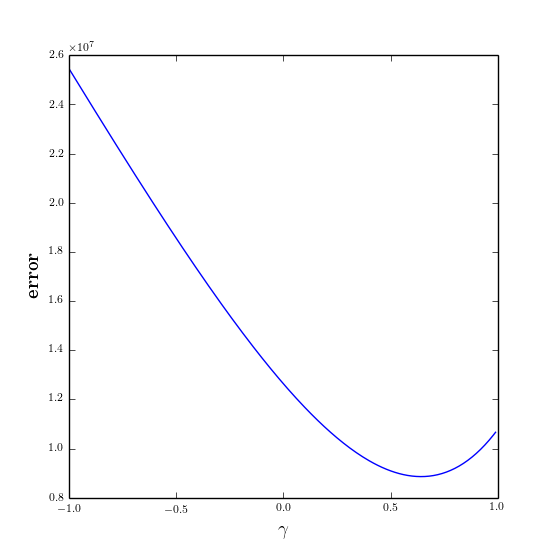
\includegraphics[width=\columnwidth]{error_V32.png}}
\subfigure{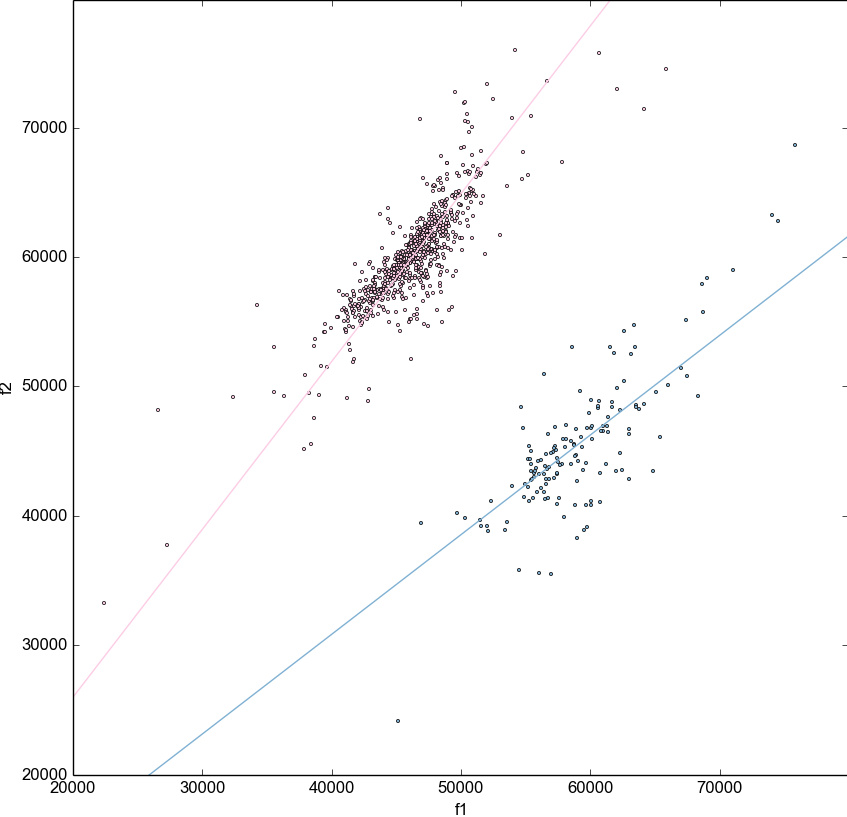
\includegraphics[width=\columnwidth]{V32.png}}
\caption{For rat V32, left shows plot of $C\left(\gamma \right)$ as a function of $\gamma$. Right shows output of clustering algorithm with $\gamma$ equal to the value shown in Fig. \ref{fig:gamma_error}.}
\end{figure*}
\end{document}

